\section{System z perspektywy użytkownika}
\label{chap:uzytkownik-gui}
Każdą funkcję realizowaną przez system można przypisać do kategorii logicznej lub kategorii zleconej. Kategoria zlecona zawiera wydarzenia, które użytkownik zainicjował poprzez integrację z panelem sterowania GUI. Kategoria logiczna zawiera funkcję, które mogą zostać wykonane, pośrednio lub bezpośrednio, jest następstwo wystąpienia wydarzeń.

Wyróznia się trzy wydarzenia: zmiana parametru progu ufności detektora obiektów poprzez manipulację suwakiem (ang. \emph{slider}), ustawienie klas obiektów wykrywanych przez detektor poprzez zaznaczenie odpowiednich przycisków przy nazwach klas oraz wybór źródła wideo z menu --- może to być jedna z kamer podłączonych do komputera lub zapisany na dysku plik wideo albo opcja wyłączenia źródła wideo. Wygląd panelu sterowania zilustrowany jest na rysunku \ref{fig:panel-sterowania}. 
Uwaga: wybór pliku wideo jako źródła należy traktować jako dodatek. W dalszej części dokumentu kamera jest jedynym rozważanym źródłem wideo.   

\begin{figure}[H]
    \centering
    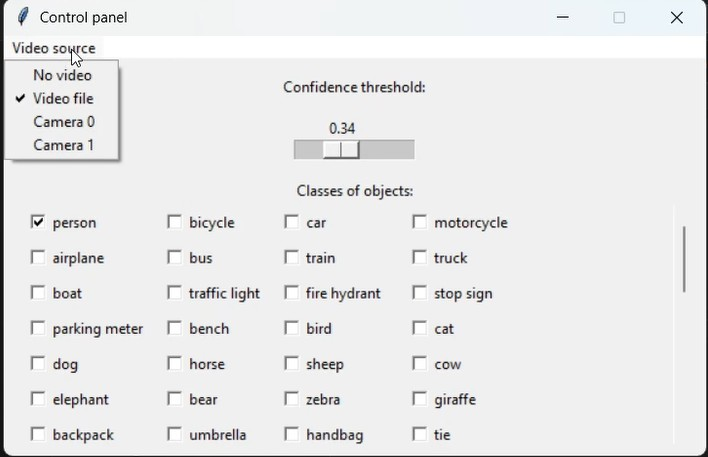
\includegraphics[width=0.79\linewidth]{r_implementacja/panel_sterowania/panel.jpg}
    \caption{Panel sterowania graficznego interfejsu użytkownika.}
    \label{fig:panel-sterowania}
\end{figure}

Zmiana parametrów detektora może odbywać się w trakcie działania zadań dektecji obiektów. Po wystąpieniu wydarzania nowe wartości parametrów nadpisują ustawienia detektora i od tego momentu tryb inferencji będzie korzystać z nowych parametrów.

Wybranie źródła wideo skutkuje uruchomieniem ustalonej sekwencji funkcji logicznych. Sekwencja ta objemuję następujące kroki:
\begin{enumerate}
    \item Pobranie klatki obrazu z wybranego źródła wideo.
    \item Detekcja ustawionych klas obiektów na bazie pobranej klatki.
    \item Jeżeli wykryto choć jeden obiekt:
    \begin{enumerate}
        \item Przetworzenie klatki w celu narysowania wygenerowanych prostokątów ograniczających. 
        \item Alarmowanie w formie dźwiękowej. 
    \end{enumerate}
    \item Dostarczenie klatki do bufora.
    \item Pobranie klatki z bufora oraz wyświetlenie jej w wyświetlaczu GUI.
\end{enumerate} 
Sekwencja jest powtarzana do momentu zakończenia się pliku wideo lub wyłączenia bądź zmiany źródła wideo. 

Na podstawie funkcji systemu zobrazowano przykładowy scenariusz wykorzystania systemu przez użytkownika z kolejnymi krokami na ryskunkach \ref{fig:mockup-2}, \ref{fig:mockup-3}, \ref{fig:mockup-4}. Przykładowe użycie to nagranie sceny ze znajdującym się człowiekiem (twarz zamazano).

\begin{figure}[H]
    \centering
    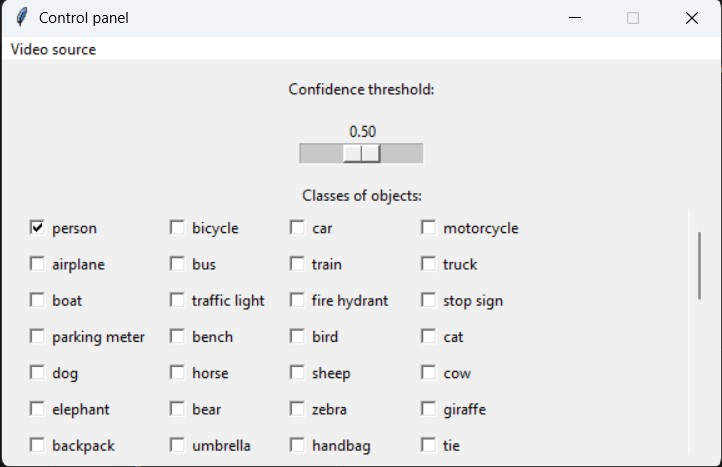
\includegraphics[width=\linewidth]{r_implementacja/panel_sterowania/panel_mockup.jpg}
    \caption{GUI w chwili uruchomienia aplikacji. Domyślne paramtry detektora to próg ufności równy 0.5 oraz klasa \emph{człowiek} jako zbiór wykrywanych klas.}
    \label{fig:mockup-2}
\end{figure}

\begin{figure}[H]
    \centering
    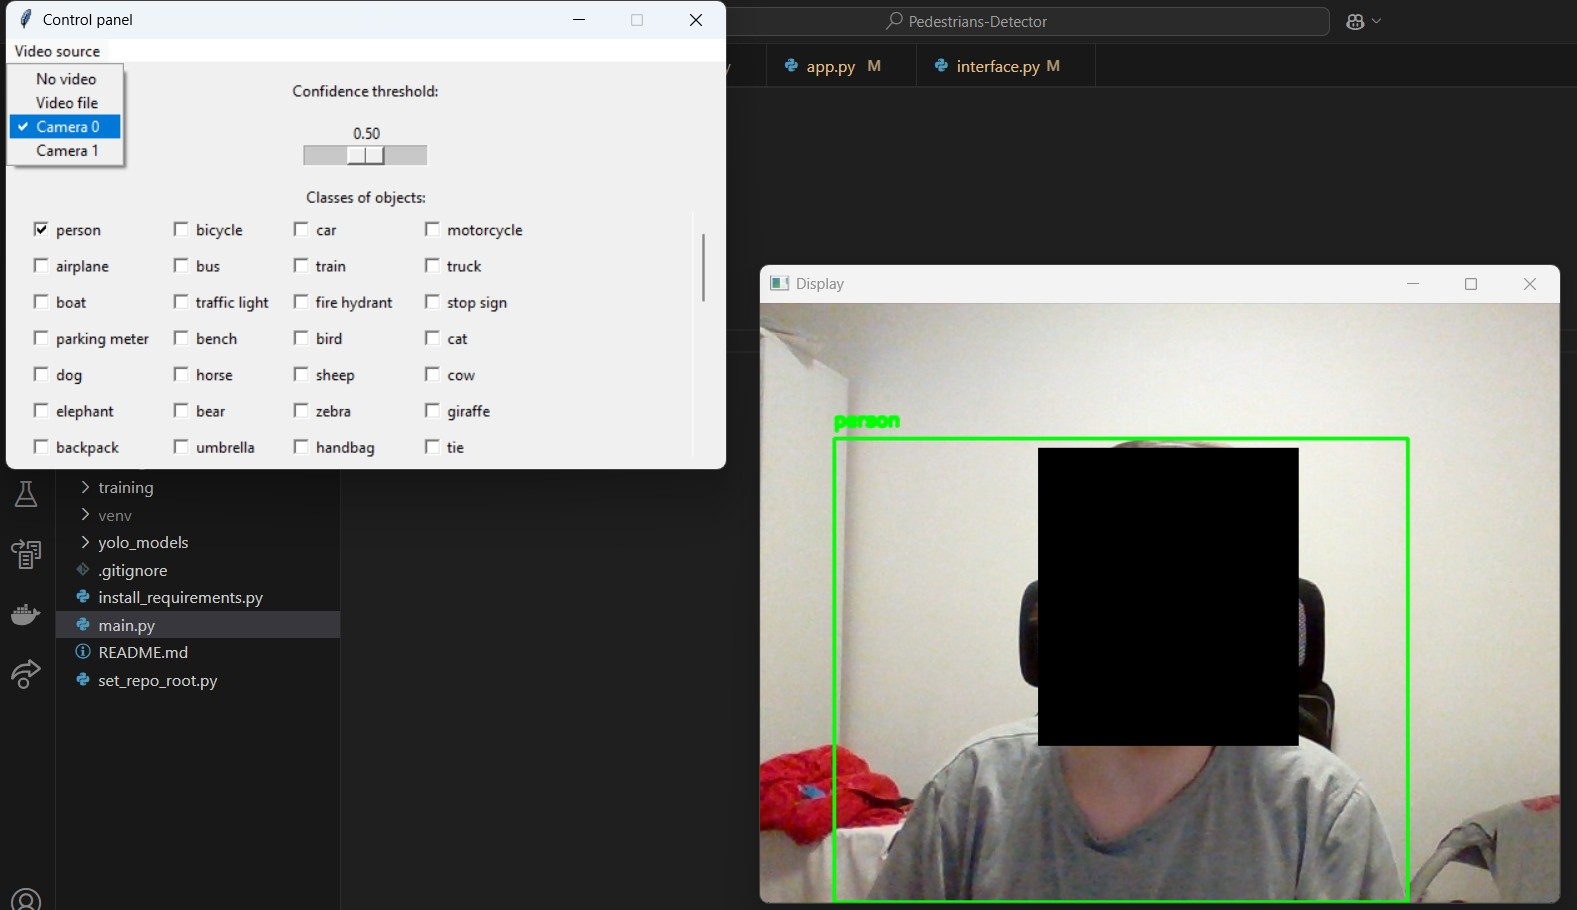
\includegraphics[width=\linewidth]{r_implementacja/panel_sterowania/camera_50.jpg}
    \caption{Uruchomienie wyświetlacza dla domyślncyh parametrów detektora oraz kamery o indeksie 0.}
    \label{fig:mockup-3}
\end{figure}

\begin{figure}[H]
    \centering
    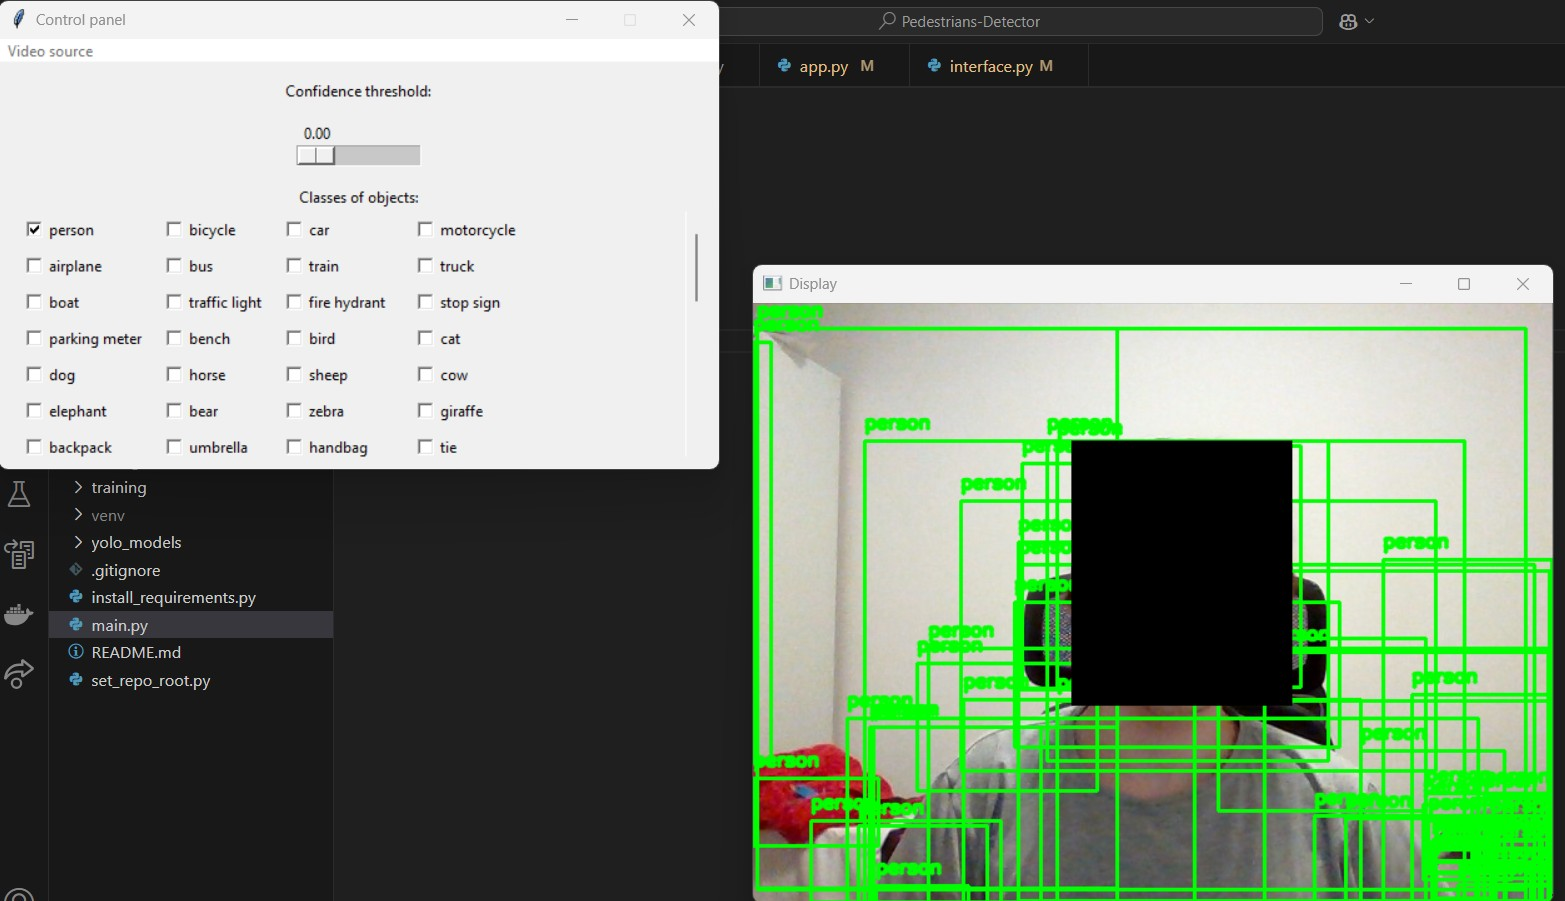
\includegraphics[width=\linewidth]{r_implementacja/panel_sterowania/camera_0.jpg}
    \caption{Zmiana progu ufności na 0.00.}
    \label{fig:mockup-4}
\end{figure}

\begin{figure}[H]
    \centering
    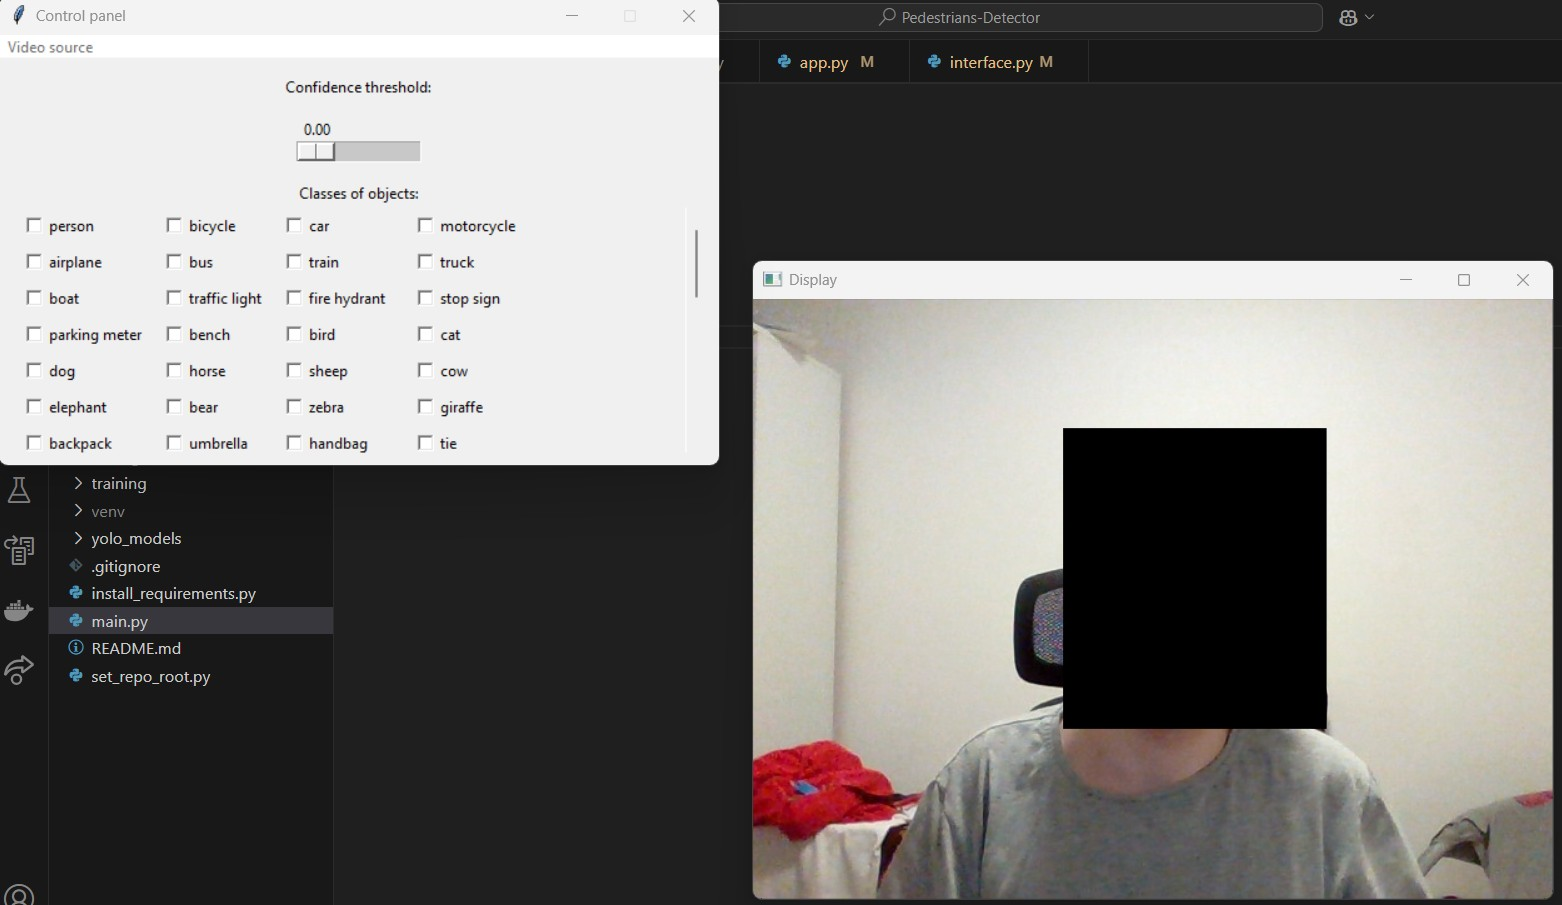
\includegraphics[width=\linewidth]{r_implementacja/panel_sterowania/camera_no_person.jpg}
    \caption{Usunięcie klasy człowiek z wykrywanych obiektów.}
    \label{fig:mockup-5}
\end{figure}
